\documentclass[12pt,a4paper]{article}

\usepackage{CJKutf8}
\usepackage[unicode,pdftex]{hyperref}
\usepackage{amsmath,amssymb,amsfonts}
\usepackage{graphicx}
\usepackage{color}
\usepackage{textcomp}
\usepackage[framed,numbered,autolinebreaks,useliterate]{mcode}

\setlength{\parindent}{0pt}
\setlength{\parskip}{18pt}

\begin{document}

\begin{CJK}{UTF8}{songti}

\title{UNFOLD}
\author{MingJian Hong \\ \texttt{hongmingjian@gmail.com}}
\date{November 7, 2011} % Activate to display a given date or no date (if empty),
         % otherwise the current date is printed
\maketitle

\textbf{Theory}

The UNFOLD recovers the image sequence from the k-t space sequence, which is under-sampled in phase direction, by labeling and resolving the overlapped components in the time axis. The idea behind UNFOLD is short and sweet, and shows that the authors had a profound understanding of the Fourier transform.

To simplify the subsequent description, the frequency-encoding direction is omitted.

With a full sampling, the DFT pair is
\begin{eqnarray}
X[k]=\sum_{n=0}^{N-1}x[n]exp(-j \frac{2 \pi}{N} nk)            \\
x[n]=\frac{1}{N}\sum_{n=0}^{N-1}X[k]exp( j \frac{2 \pi}{N} nk)
\end{eqnarray}
Suppose that the $N$ is even, two under-sampling patterns are defined as follows.
\[ 
\delta_{o}[n] = \left\{ \begin{array} 
                 {r@{\quad:\quad}l}
                 1 & n = 2k+1 \\  0 & n = 2k
                 \end{array}  \right.  \]
\[ 
\delta_{e}[n] = \left\{ \begin{array} 
                 {r@{\quad:\quad}l}
                 0 & n = 2k+1 \\  1 & n = 2k
                 \end{array}  \right.  \]
where k $\in [0, \frac{N}{2}-1]$

Obviously, $\delta_{o}[n]=\delta_{e}[((n-1))_N]$ holds true. According to the property of the DFT, we have 
\begin{equation}
IDFT(\delta_{o})[n]=IDFT(\delta_{e})[n]exp(j\frac{2 \pi}{N}n)
\end{equation}
The $IDFT(\delta_{e})$ can be expanded as follows.
\begin{eqnarray}
IDFT(\delta_{e})[n] & = & \frac{1}{N}\sum_{k=0}^{N-1}\delta_{e}[k]exp(j\frac{2 \pi}{N} kn) \nonumber\\
                    & = & \frac{1}{2}\frac{1}{N/2}\sum_{k=0}^{N/2-1}exp(j\frac{2 \pi}{N/2} kn)
\end{eqnarray}
which is reduced to 
\begin{equation} 
IDFT(\delta_{e})[n] = 
\left\{ 
      \begin{array} 
      {r@{\quad:\quad}l}
      \frac{1}{2} & n = 0, \frac{N}{2} \\
      0           & otherwise
      \end{array}
\right.
\end{equation}
by using the equation in the Problem 3.54 of [3]. Accordingly, we have
\begin{equation}
IDFT(\delta_{o})[n]=
\left\{ 
      \begin{array} 
      {r@{\quad:\quad}l}
       \frac{1}{2} & n = 0 \\
      -\frac{1}{2} & n = \frac{N}{2} \\
       0           & otherwise
      \end{array}
\right.
\end{equation}
The reconstructions from the k-space under-sampled by $\delta_{e}[n]$ and $\delta_{o}[n]$ are as follows.
\begin{eqnarray}
x_{e}[n] & = & IDFT(X\delta_{e}) \nonumber\\
         & = & IDFT(X)*IDFT(\delta_{e})
\end{eqnarray}
\begin{eqnarray}
x_{o}[n] & = & IDFT(X\delta_{o}) \nonumber\\
         & = & IDFT(X)*IDFT(\delta_{o})
\end{eqnarray}
Based on the property of the convolution, $x_{e}[n]$ and $x_{o}[n]$ are the sum of replications of $\frac{1}{2}x[n]$ and $\frac{(-1)^{k}}{2}x[n]$ centered at $k \frac{N}{2}, k=0, \pm1, \pm2, ...$, respectively, as shown in Fig.(\ref{replications}).
\begin{figure}
\centering
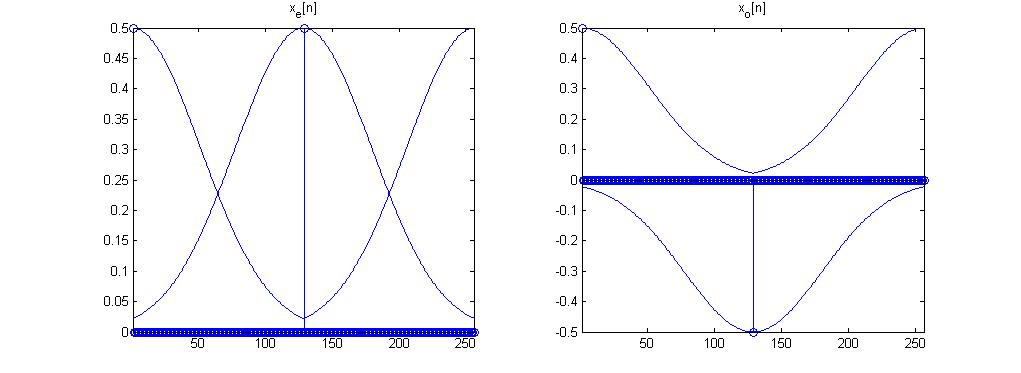
\includegraphics[scale=.5]{replicates}
\caption{replications - $x_e$[n] and $x_o$[n] is the sum of two curves.}
\label{replications}
\end{figure} 
Mathematically, we have
\begin{eqnarray}
x_{e}[n]=\frac{1}{2}(x[n]+x[((n+\frac{N}{2}))_N]) \\
x_{o}[n]=\frac{1}{2}(x[n]-x[((n+\frac{N}{2}))_N])
\end{eqnarray}
So far, we do not consider the time axis of the image sequence. Suppose that the k-space of the even frame is under-sampled by $\delta_{e}$ and odd frame by $\delta_{o}$. 

If the points at $n_0$ and $n_1=((n_0+\frac{N}{2}))_N$ are constant in time, the value of aliased point where they overlap will oscillate between $\frac{1}{2}(x[n_0]+x[n_1])$ and $\frac{1}{2}(x[n_0]-x[n_1])$ frame by frame, as shown in the Fig.(\ref{unfold}a).
\begin{figure}
\centering
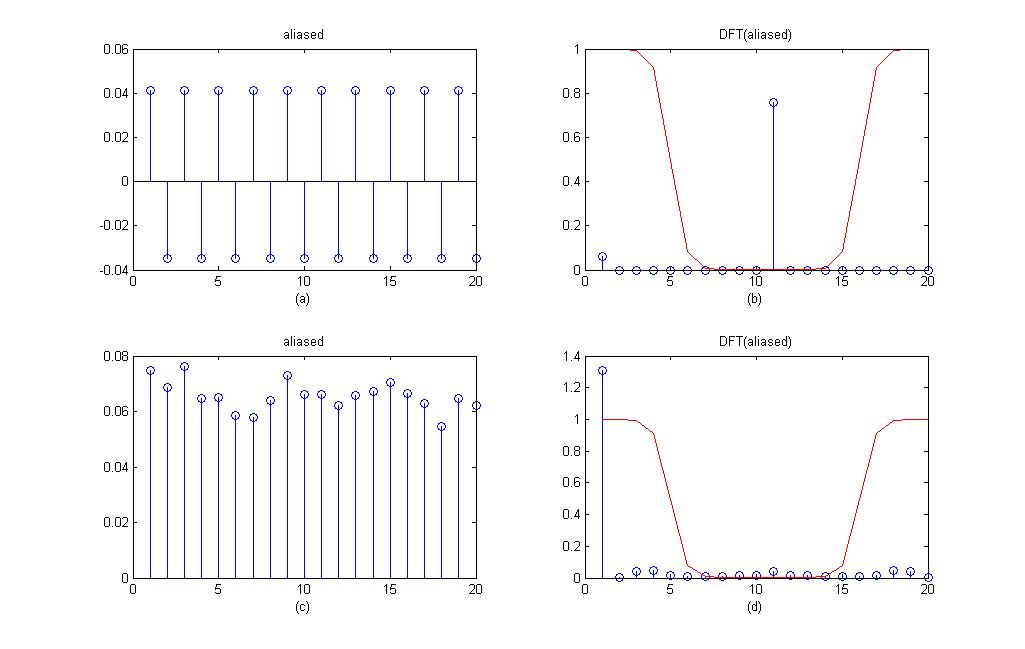
\includegraphics[scale=.5]{unfold.jpg}
\caption{UNFOLD}
\label{unfold}
\end{figure} 

The UNFOLD resolves $x[n_0]$ and $x[n_1]$ out of the aliased point by Fourier transform in the time axis. As shown in the Fig.(\ref{unfold}b), the spatial overlapped points are discriminable in the Fourier domain along the time axis. By applying a predefined filter (the red curve), the $x[n_0]$ and $x[n_1]$ can be separated and recovered.

In the case of non-constant $x[n_0]$ and $x[n_1]$ in time (Fig.(\ref{unfold}c)), the spectra associated with them contains a range of frequencies instead of a single component, as shown in the Fig.(\ref{unfold}d).


\medskip
\textbf{Matlab code for UNFOLD}
\lstinputlisting{unfold.m}

\textbf{References}

[1] B. Madore, G. H. Glover, and N. J. Pelc, "Unaliasing by Fourier-encoding the overlaps using the temporal dimension (UNFOLD), applied to cardiac imaging and fMRI", Magnetic Resonance in Medicine 42, no. 5 (1999): 813-828.

[2] Jeffrey Tsao, "On the UNFOLD method", Magnetic Resonance in Medicine 47, no. 1 (2002): 202-207.

[3] A. V. Oppenheim, A. S. Willsky, and  with S. Hamid, Signals and Systems, 2nd ed. Prentice Hall, 1996.

%\bibliographystyle{amsplain}
%\bibliography{chemo}

\end{CJK}
\end{document}
